% !TEX root =  ../report.tex
% !TeX spellcheck = en-GB

\section{Evaluation}
\label{s:eval}

This project was intended as an investigation, and therefore it can certainly be considered successful. The potential for optimisation through JIT compilation has been proved, via the demonstration that the optimisation of defining constants as literal values is able to re-coup the cost of run-time compilation if the problem size is sufficiently large.
\par
Since the space for optimisation by this technique is relatively small, the problem size does have to be very large to see benefit, however HPC applications do tend to be very large, hence why they are not run on normal computers, so this is not a significant restriction.
\par
Through the contributions made to the OP2 project while completing this project, important groundwork has been laid for future contributors to build on top, and implement further optimisations and run-time assertions which might achieve further speedup at run-time.

\subsection{Future Work}
\label{ss:fw}

\subsubsection{Run-Time Assertions}
As previously mentioned, it seems necessary for more to be assertions to be made at run-time in order to produce more effective speed-up after JIT compilation. \par
There are a number of possible loop optimisations which could be made, including identifying a loop inside a kernel, and at run-time having the loop bound be hard-coded to remove the need to evaluate the expression of every iteration; or more complex optimisation where two separate parallel loops might be provably able to be fused into a single loop, but only if the inputs allow for it - meaning this could only be done at run-time.

\noindent There is also research into applying loop tiling to the generated code, which is dividing the iterations of a loop into sub-regions where both temporal and spatial locality in memory can be exploited. \par

\begin{wrapfigure}{r}{.4\textwidth}
  \centering
  \caption{2D Loop Tiling}
  \label{fig:tile2D}
  \hspace{-1em}
  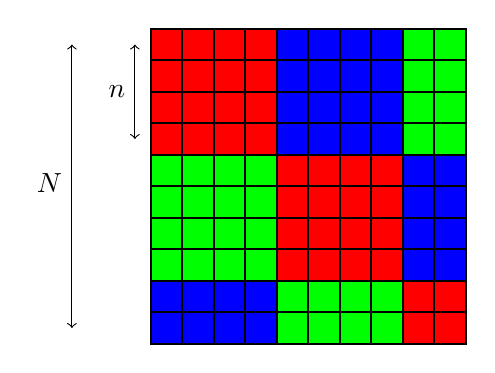
\begin{tikzpicture}
      [%%%%%%%%%%%%%%%%%%%%%%%%%%%%%%
          box/.style={rectangle,draw=black,thick, minimum size=.4cm},
          scale=0.4
      ]%%%%%%%%%%%%%%%%%%%%%%%%%%%%%%

  \foreach \x in {0,...,9}{
      \foreach \y in {0,...,9}
          \node[box] at (\x,\y){};
  }

  \foreach \x in {0,...,3}{
      \foreach \y in {6,...,9}
        \node[box,fill=red] at (\x,\y){};
  }

  \foreach \x in {4,...,7}{
      \foreach \y in {6,...,9}
        \node[box,fill=blue] at (\x,\y){};
  }

  \foreach \x in {8,...,9}{
      \foreach \y in {6,...,9}
        \node[box,fill=green] at (\x,\y){};
  }

  \foreach \x in {0,...,3}{
      \foreach \y in {2,...,5}
        \node[box,fill=green] at (\x,\y){};
  }

  \foreach \x in {4,...,7}{
      \foreach \y in {2,...,5}
        \node[box,fill=red] at (\x,\y){};
  }

  \foreach \x in {8,...,9}{
      \foreach \y in {2,...,5}
        \node[box,fill=blue] at (\x,\y){};
  }

  \foreach \x in {0,...,3}{
      \foreach \y in {0,...,1}
        \node[box,fill=blue] at (\x,\y){};
  }

  \foreach \x in {4,...,7}{
      \foreach \y in {0,...,1}
        \node[box,fill=green] at (\x,\y){};
  }

  \foreach \x in {8,...,9}{
      \foreach \y in {0,...,1}
        \node[box,fill=red] at (\x,\y){};
  }

  \draw[<->] (-1,6) -- (-1,9);
  \node[anchor=south east] at (-1,7) {$n$};
  \draw[<->] (-3,0) -- (-3,9);
  \node[anchor=south east] at (-3,4) {$N$};

  \end{tikzpicture}
\end{wrapfigure}
For example, a loop iterating over a 2D array of size $N \times N$, with Level 1 (L1) cache size of $n$, such that $n < N$, would benefit from dividing the array into squares of size at most $n \times n$ (see Figure \ref{fig:tile2D}), as long as this does not violate any data dependencies in the order of operations. Doing so prevents values from being evicted from L1 cache prior to being needed again.\par
Currently this has only been applied to OPS \cite{opstiling}, the precursor to OP2 \cite{opsmain}, which supports structured mesh solvers only. There does exist a 2019 paper \cite{slope} on automated loop tiling for unstructured meshes, and the issues posed by the need for indirect array accesses. A library provided which demonstrates the technique \cite{SLOPErep}, including a demo using the same \textit{airfoil} application used for this report.
\par
During this project it was suggested that applying loop tiling inside the JIT compilation stage could be a good extension, and would likely provide speedup, however unfortunately there was not sufficient time to reasonably expect the functionality to be finished.

\subsubsection{CUDA JIT Compilation}
Going in a different direction, the CUDA library does provide an interface for JIT compilation natively, which would allow for re-compilation without requiring a system call to \verb|make| for every loop kernel. System calls can be a significant bottleneck in some cases, and this problem would only compound for applications with a large number of parallel loops. Therefore, using the CUDA JIT compilation system would likely bring down the upfront cost of recompilation. For \textit{airfoil} this re-compile time is very low, it would not have much impact on the results gathered.
\par
Using CUDA's native JIT compilation pipeline would provide the added benefit that a application developer using OP2 would not have to write the Makefile themselves, as currently its contents are not generated by the OP2 code generator, but simply relies on the executable producing an error if a Makefile with the correct target does not exist.

\subsubsection{Alternative Hardware Targets}
Finally, there are other hardware targets supported by OP2 which may be able to benefit from Just-In-Time compilation, and since the purpose of OP2 is to provide performance on multiple hardware platforms from a single application code any new optimisation which is found to improve performance, should also be ported to other platforms where it might be able to provide benefit. Any users who do not  primarily utilise NVidia GPU hardware should benefit from the JIT compilation optimisation.

\clearpage
\subsection{Project Management}
\label{ss:pm}
This Section serves as a reflection on the project as a whole, and how I believe it went.
\par
The Gantt chart in figure \ref{progGantt} was produced for the progress report submitted in November, 6 weeks into the project. Having now completed the project I can reflect on how well the timeline was followed, and the successes and challenges of each of the four periods.
\newcommand\w{25}
\begin{figure}[h]
\centering
\caption{\label{progGantt} Gantt Diagram produced with Progress Report}
\makebox[0pt]{
\begin{ganttchart}[
expand chart=1.22\textwidth,
vgrid={*{1}dotted, *4{white},*1{dotted}, *{12}{white}, *1{dotted}, *1{white}, *1{dotted}, *5{white}},
hgrid=true,
y unit chart=0.8cm,
inline,
today=6,
today label=Progress Report,
today label font=\itshape,
]{0}{\w}

 \gantttitle{Timeline}{26} \\
 \gantttitlelist{0,...,\w}{1} \\

 \ganttgroup{Research}{1}{5} \\ %0%

 \ganttset{inline=false}
 \ganttbar{Read Papers}{1}{2}          %1%
 \ganttset{inline=true}

 \ganttgroup{Implementation}{6}{18} \\ %2%

 \ganttset{inline=false}
 \ganttbar{Familiarity Work}{2}{5}     %3%
 \ganttset{inline=true}

 \ganttgroup{Benchmarking}{19}{20} \\  %4%

 \ganttset{inline=false}
 \ganttbar{Feature Development}{6}{8}  %5%
 \ganttbar{} {10}{12}                   %6%
 \ganttbar{} {14}{17}                  %7%
 \ganttset{inline=true}
 \ganttgroup{Documentation}{21}{25} \\ %8%

 \ganttset{inline=false}

 \ganttbar{Feature Testing}{9}{9}      %9%
 \ganttbar{}{13}{13}                   %10%
 \ganttbar{}{18}{18}                   %11%

\\

 \ganttbar{Results Gathering}{19}{19}  %12%
 \\
 \ganttbar{Results Processing}{19}{20} %13%
 \\

 \ganttbar{Final Report}{21}{25} \\    %14
 \ganttbar{Presentation}{21}{22}       %15

 \ganttlink{elem1}{elem3}
 \ganttlink{elem3}{elem5}
 \ganttlink{elem5}{elem9}
 \ganttlink{elem9}{elem6}
 \ganttlink{elem6}{elem10}
 \ganttlink{elem10}{elem7}
 \ganttlink{elem7}{elem11}
 \ganttlink{elem11}{elem12}
 \ganttset{link mid=0.25}
 \ganttlink{elem11}{elem13}
 \ganttset{link mid=0.5}
 \ganttlink{elem13}{elem14}
 \ganttset{link mid=0.25}
 \ganttlink{elem13}{elem15}
 \ganttset{link mid=0.5}
\end{ganttchart}
}
\end{figure}

\subsubsection{Challenges and Reflection}
\hspace{\parindent} \minititle{Research}
The research section of my project involved reading scientific papers, many produced by contributors to the OP2 framework; as well as working hands-on with both CUDA and OP2 to try to build familiarity before the actual implementation began. On reflection, my research was mostly focused on the existing OP2 work, and many of my sources were from the same authors. Once I had already decided on my approach and begin implementation I discovered some similar work which might have influenced the direction of the project if I had been aware of them earlier on.
\par
Considering that I had never written code for a graphics card before starting this project, I am happy with the confidence in using the CUDA programming model I have built. The time I had allotted to research did need to be extended from the plan at the outset of the project, as after three weeks I was not confident enough with the existing OP2 code base to begin making an addition. The additional two weeks were sufficient more me to feel able to begin the implementation.

\minititle{Implementation}
The Implementation progressed largely as expected, with progress made at a good pace for the time allocated. I did find that while the timetable above listed a total of 3 full weeks for testing, partial solutions were difficult to test fully by as there was no executable generated to ensure the result was correct or perform much benchmarking until towards the end of the implementation.
\par
Instead testing during implementation relied more on comparing expected results from the code generation of airfoil, and modified versions of airfoil, with the actual outputs of the code generation scripts. For some areas of development, I found it useful to write the code manually into the airfoil files, and figure out how it could work by compiling the manually written code. Once it was compiling successfully, the code generator could be modified to produce equivalent code, but with application specific names replaced with variables so that it would work for any application.
\par
I discussed with my supervisor some extension work which could have been a part of the implementation if there was time, such as the Loop Tiling feature mentioned in previous Section \ref{ss:fw}. Since the core functionality of the project was only completed with 2 weeks of planned implementation time left, it was decided that this unlikely to be completed in the time frame, and that it would be better to thoroughly benchmark the completed functionality than to attempt a complex extension feature and potentially leave it incomplete.

\minititle{Benchmarking}
It was fortunate for the project as a whole that the decision to move on to benchmarking instead of pursuing further functionality was taken, as the original plan allotted only a week for gathering results and a second for analysing the results. In reality, the extra 2 weeks that had been allocated Implementation to were also required, as well as an additional week intended for making the project presentation.
\par
The delay was mostly due to the desire to use a HPC cluster to gather proper benchmarking data. While the graphics card in my personal laptop was sufficient for validating the code executed correctly, the results would likely have been noisy and inconsistent if not gathered on a dedicated system. Finding a cluster that could allow me access to a Kepler generation GPU, and getting familiar with using the system once accepted took longer than expected. With the benefit of hindsight it is clear that this process should have begun much earlier in the project, as from the start it was always going to be necessary to have access to a HPC cluster.
\par
Eventually the Cambridge Service for Data-Driven Discovery (CSD3) kindly approved me to use their \textit{Wilkes2} GPU cluster, with workloads I submitted being placed in a low priority queue. This provided its own challenge, as I often had to wait overnight for results of a submitted job to be provided, or to find out it failed with some error. I was already starting to become familiar with SLURM from using it as part of a High Performance Computing module, and my knowledge only improved for needing to make use of it here as well.

\minititle{Documentation}
The last period of work is producing the documentation, which encompasses both creating and giving a presentation on the completed work, and writing this report. The presentation was made using google slides, and I believe it went well, although the demonstration was perhaps not as thorough as it should have been. The results I collected for the presentation were only for 10,000 time steps, while the results in this report where for 1,000,000 - which gave a much better indication of the outcome of applying the optimisation. The total execution time of the application increased from ~30 seconds to ~40 minutes, which allows a small change to amplify into a noticeable difference.
\par
This report produced as the final submission utilises LaTeX and BibTeX, and also was completed well within the allotted time, allowing for sufficient re-drafting. The two week extension provided to account the current pandemic was helpful to make the final stages of the report less stressful to write.

\subsubsection{Tools Selection}
I am satisfied with my selection of tools for this project. There was certainly no need to diverge from using GitHub for version control as the rest of the OP2 Framework does, and there have been no issues with using it during this project as I was already very familiar with using \verb|git| prior to starting. Since there was no collaboration, the workflow is simple as there is only a single branch, with commits whenever a feature or fix is completed.
\par
For development, the use of GNU make for AOT compilation is fine enough and very convenient to combine many commands into a single simple one, however, using it for the JIT compile as well is not an ideal interface for an application developer using OP2, as they would need to recreate the contents of my Makefile themselves. It also relies on the OP2 library files, the generated code and the Makefile all being accessible by the binary at run-time, which might not always be the case.
\par
Code was mostly written using Atom \cite{atom} as a text editor, or Vim \cite{vim} when working remotely on the HPC cluster. Atom allows multiple files to be open at once, so the results of code generation can be seen immediately, and also allows generated code from my code generation to be compared quickly with that from existing translation scripts. I used Vim when only a terminal is available because it is the editor I am most familiar with in that context, and because its popularity means it is usually already available on Linux systems.
\par
Lastly, Google Sheets \cite{gsheets} was selected for the presentation because of familiarity, and to ensure changes are automatically saved to a remote in case of loss of data. I prefer LaTeX for producing reports as it allows greater control of the structure of the document than other editors, and provides access to TikZ \cite{tikz}: a powerful package used for producing diagrams.
